% !TeX root = Tesis.tex
% !TeX encoding = UTF-8
% !TeX spellcheck = es_CU-SpanishCuba
\chapter{Diagrama de tres atractores}
\label{cap2}
\onehalfspacing


\section{El diagrama de N + GB + EA}\label{sec:ngbad}

Nuestro punto de partida es el diagrama de los datos de expresión genética del análisis de componentes principales para la materia blanca del cerebro, mostrado en la Fig. \ref{fig:fig1a}. Como se puede notar en la figura, las dos primeras componentes principales capturan más del 80 \% de la varianza del sistema. Por lo tanto, es una representación bidimensional adecuada de la distribución real de los puntos en el espacio de expresión genética.

\begin{figure}[!htb]
	\centering
	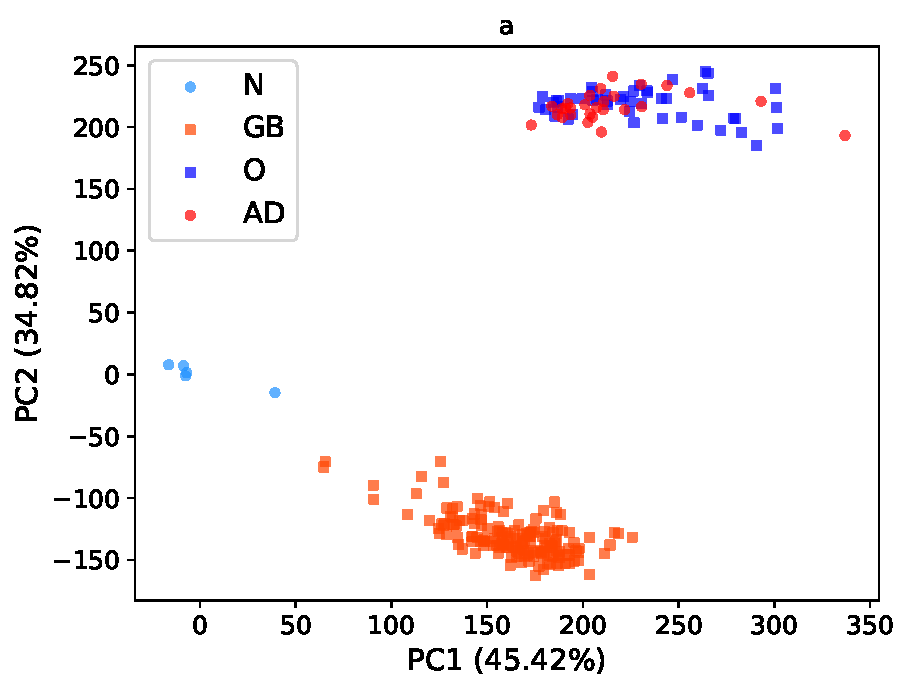
\includegraphics[width=0.75\linewidth]{figures/Fig_1a.pdf}
	\caption{\label{fig:fig1a}
		Análisis de componentes principales para los datos de expresión genética.}
\end{figure}

En la figura se pueden apreciar 4 grupos de muestras. Las muestras marcadas como N y GB corresponden, a especímenes patológicamente normales y tumorales en los datos del TCGA para el glioblastoma \cite{Brennan_2013}. Los centros de las nubes de muestras de N y GB en el espacio de expresión genética definen, respectivamente, los atractores Normal (homeostático) y Glioblastoma de Kauffman \cite{Huang_2009, Gonzalez_2023}. De hecho, la acumulación de puntos en una determinada región de este espacio indica que esta es un atractor de la red de regulación Genética que gobierna la dinámica del sistema.

Por otro lado, los grupos etiquetados como EA y O corresponden a las muestras de la materia blanca del cerebro de la enfermedad del Alzheimer y del grupo de control (\textit{old}) en el estudio del Instituto Allen \cite{Miller_2017}. 

La Fig. \ref{fig:pcaotoad} es una reconstrucción de la figura 3a de la referencia \cite{Gonzalez_2021}. En esta se muestran los resultados del PCA para los datos de expresión genética de la materia blanca del cerebro del Instituto Allen. La primera componente principal (PC1), la cual contiene el $24.7 \%$ de la varianza total, discrimina entre las muestra de O y EA. La posición del centro de la nube de O en este eje es $\left\langle x_1 \right\rangle  = 0 $, y para la EA es $\left\langle x_1 \right\rangle = 40.97 $. Sin embargo, los radios de las nubes de las muestras de O y EA son más grandes que la distancia entre los centros, que son $80.69$ y $72.64$ respectivamente.
%\alert{Estudiamos la transición de O hacia EA en la referencia \cite{Gonzalez_2021}}. En la Fig. \ref{fig:otoad}

\begin{figure}[!htb]
	%TODO:
	\centering
	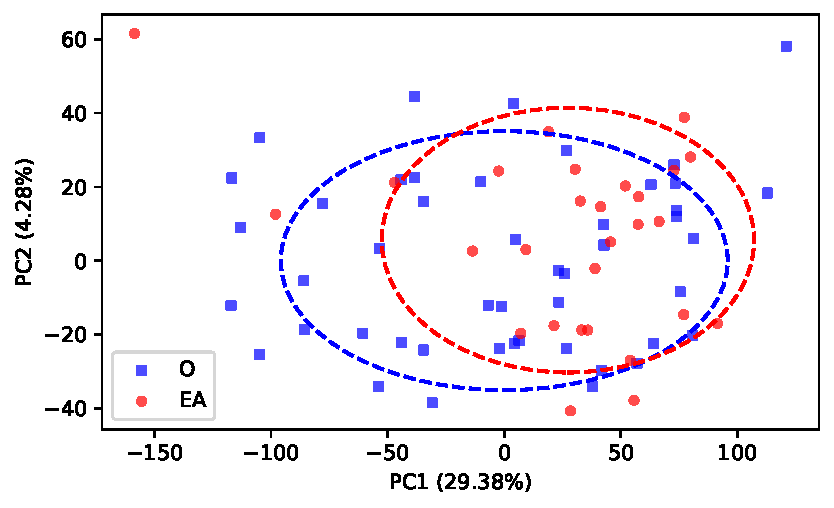
\includegraphics[width=0.75\linewidth]{figures/pca_o_to_ad_1}
	\caption{ Análisis de componentes principales de los datos de expresión genética del Instituto Allen de la materia blanca del cerebro. Se representan las muestras de O y la EA. Las elipses discontinuas se dibujan de acuerdo con las desviaciones estándar de cada conjunto. Tomada de la referencia \cite{Gonzalez_2021}.}
	\label{fig:pcaotoad}
\end{figure}

Es bien conocido el papel de la edad en la EA, especialmente en ancianos \cite{alz2019}. Por lo tanto, podemos usar la edad como una variable de tiempo para seguir la transición. A pesar del número relativamente pequeño de muestras, se realizó un análisis de regresión lineal de la posición media de $\left\langle x_1 \right\rangle$ en función de la edad en las muestras de O, Fig. \ref{fig:otoad}. Esta figura es una reproducción de la 4a de la referencia \cite{Gonzalez_2021} y en la cual se ilustra que $\left\langle x_1 \right\rangle = -287.12 + 3.24 \cdot edad$. En las muestras de la EA, sin embargo, no se encontró correlación entre $\left\langle x_1 \right\rangle$ y la edad observada. Por lo tanto, la posición de la zona EA es aproximadamente fija, y la nube de muestras de O evidencia una deriva hacia el mínimo de la EA a medida que aumenta la edad.

\begin{figure}[!htb]
	\centering
	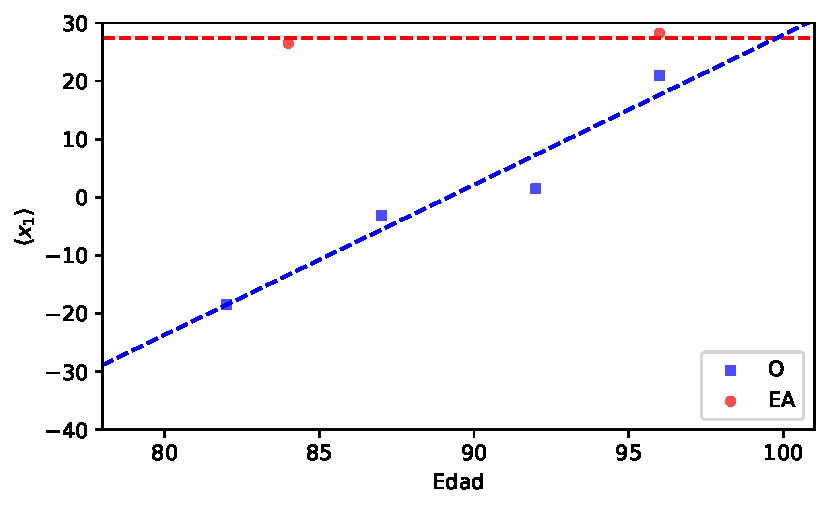
\includegraphics[width=0.75\linewidth]{figures/O_to_AD_1}
	\caption{Posición media de la muestra a lo largo del eje PC1 en función de la edad. A medida que aumenta la edad, las muestras de O experimentan una deriva hacia la región de la EA, cuyo centro es aproximadamente independiente de la edad. Tomada de la referencia \cite{Gonzalez_2021}.}
	\label{fig:otoad}
\end{figure}

Una mejor ilustración de este hecho viene representada en la Fig. \ref{fig:supplotoad}, donde se compara la densidad de probabilidad de las muestras de O y de la EA. Esta reproduce la imagen S2 del material suplementario de la referencia \cite{Gonzalez_2021}. Para construir dicha figura, se definieron cuatro intervalos de edades, que contienen aproximadamente la misma cantidad de muestras de O: [77, 84], [84, 90], [90, 95], [95, 100+]. La probabilidad total de las muestras de la EA es mostrada en los cuatro paneles. El solapamiento creciente entre las densidades de probabilidad evidencia una transición gradual de las muestras del grupo O hacia valores característicos del grupo EA.

\begin{figure}[!htb]
	%TODO: hacer un replot de la figura
	\centering
	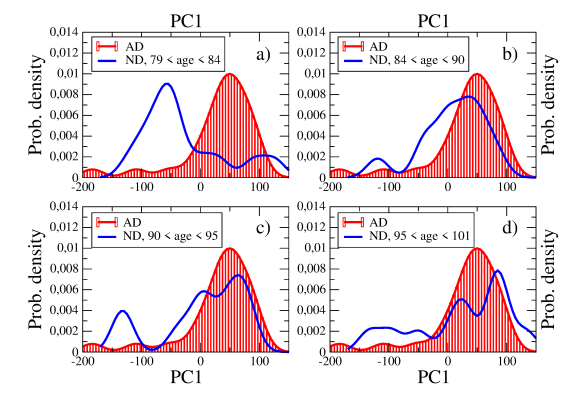
\includegraphics[width=\linewidth]{figures/suppl_otoad}
	\caption{Densidad de probabilidad de las muestras de O y de la EA a lo largo del eje de PC1. Cada panel es para un intervalo de edad para las muestras de O. La probabilidad de la EA, la cual es aproximadamente independiente de la edad, es mostrada en los cuatro paneles. Tomada de la referencia \cite{Gonzalez_2021}.}
	\label{fig:supplotoad}
\end{figure}

Esta propiedad sugiere que el centro de la nube de muestras de la EA define un atractor en el espacio de expresión genética. Las muestras de O parecen ser atrapadas por el atractor de la EA en el proceso del envejecimiento.

Así, en nuestra aproximación, obtenemos un panorama en el espacio de expresión genética de tres atractores: N, GB y EA, y un conjunto de muestras de O que se desplaza hacia la EA. Las posiciones relativas y las principales transiciones entre los atractores se resumen en la Fig. \ref{fig:fig1b}. Asumimos que estas transiciones están determinadas por la biología subyacente a los procesos en los tejidos. La transición de N a la EA se denomina ``EA anticipada'' para enfatizar que también existe una vía hacia la EA a través del envejecimiento: ``EA tardía''. La figura también indica una vía para el GB y para el envejecimiento.

\begin{figure}[!htb]
	\centering
	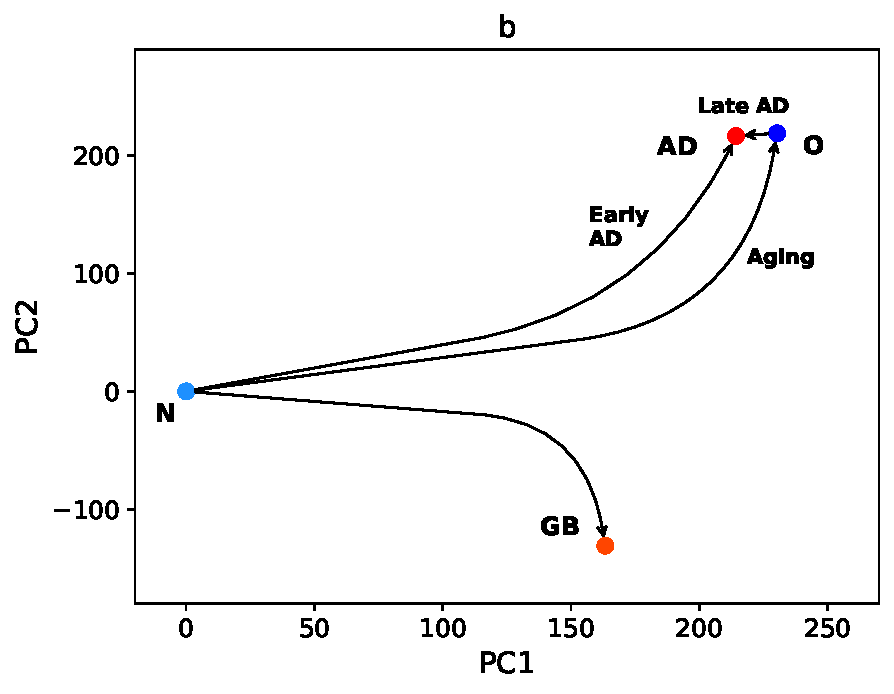
\includegraphics[width=0.75\linewidth]{figures/Fig_1b.pdf}
	\caption{Posiciones relativas y principales transiciones entre los atractores.}
	\label{fig:fig1b}
\end{figure}

\section{Panorama del \textit{fitness}}\label{sec:sec22}

Existe información cualitativa que puede introducirse en nuestra descripción. Esta se relaciona con una variable de \emph{fitness}, de modo que dibujamos una especie de diagrama de Wright \cite{wright1932roles}. En la Fig. \ref{fig:fig1c} se muestra un diagrama esquemático que contiene un gráfico de contorno hipotético del \emph{fitness}. Los atractores N y GB son máximos de \emph{fitness} y deberían estar separados por una barrera de bajo \emph{fitness} \cite{Gonzalez_2021}. El GB debería ser el máximo más alto de los tres actores representados \cite{Gonzalez_2021, gonzalez2022estimating}. Por otro lado, la transición de O a la EA es casi continua, con un número relativamente pequeño de genes expresados diferencialmente \cite{Gonzalez_2021}. Esto significa que existe una barrera muy pequeña, o incluso una ruta sin barrera, que conecta a O y a la EA. Esperamos una barrera de bajo \emph{fitness} que impida las transiciones directas de N a la EA, y un máximo de la EA pequeño, ya que este atractor se encuentra en la región de bajo \emph{fitness}, lejos de N. 

\begin{figure}[!htb]
	\centering
	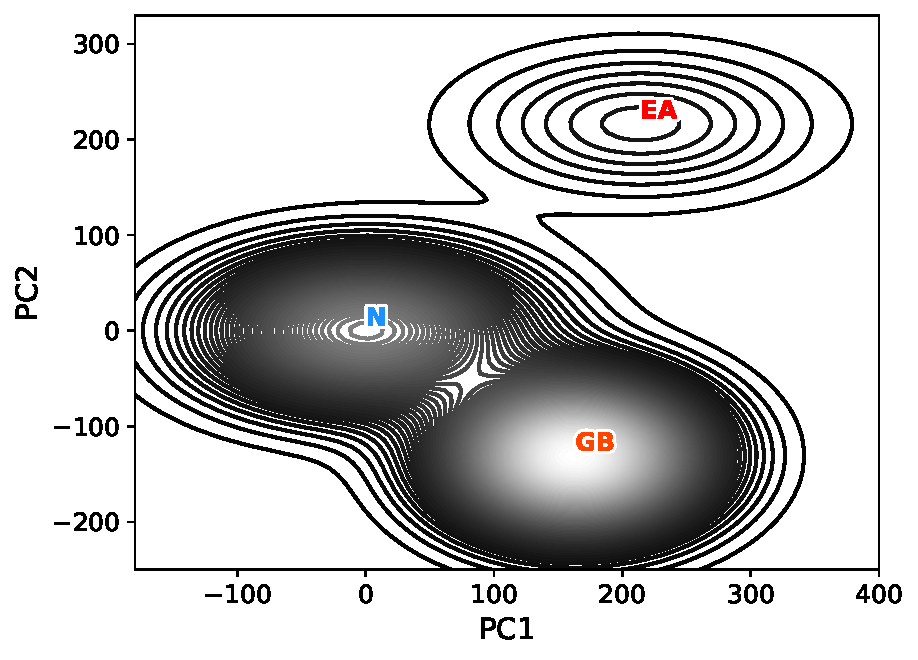
\includegraphics[width=0.75\linewidth]{figures/Fig_1c.pdf}
	\caption{Diagrama de Wright que muestra un gráfico de contorno hipotético del \emph{fitness}. El máximo absoluto corresponde con el estado de GB. El atractor de la EA se representa como un ligero máximo local.}
	\label{fig:fig1c}
\end{figure}

Todos estos hechos se representan en la Fig. \ref{fig:fig1c}. El esquema se construye a partir de una suma de gaussianas centradas en los atractores, con desviaciones estándar proporcionales a los valores reales observados en la Fig. \ref{fig:fig1a} y con alturas que respetan cualitativamente la fuerza relativa de los atractores.

Resaltemos el significado de un diagrama de Wright en el tejido cerebral. En otros tejidos, la evolución somática se relaciona principalmente con la replicación de células madre. Sin embargo, en su estado normal, el cerebro es un tejido de replicación muy lenta \cite{spalding2005retrospective}. Los cambios en pequeñas regiones cerebrales, es decir, los desplazamientos en el diagrama, son básicamente daños acumulados, es decir, envejecimiento \cite{schumacher2021central}. Sin embargo, una vez que se produce la transición al estado GB, se produce un enorme aumento de la tasa de replicación de las células tumorales. Observemos, además, que los cambios relacionados con el envejecimiento son muy evidentes en la sustancia blanca \cite{guttmann1998white}.


\section{Limitaciones}\label{sec:limitations}

En este trabajo se utilizaron datos de expresión genética, en formato FPKM, de las referencias \cite{Brennan_2013, Miller_2017}. Estos fueron obtenidos usando diferentes plataformas. Nosotros tomamos aproximadamente 30 000 genes que están perfectamente identificados en ambas plataformas y realizamos un sencillo análisis de componentes principales \cite{Lever2017}, como se definió en la sección \ref{subsec:svd}. Para definir los valores de la expresión diferencial logarítmica y calcular la matriz de covarianza utilizada para el PCA, se utilizó como referencia común la media geométrica en el conjunto de muestras N.

Debido al uso de estos datos, proveniente de dos experimentos distintos, para realizar un solo calculo de PCA surgen problemas tanto técnicos como conceptuales. Por ejemplo, la referencia N corresponde precisamente al estado normal del cerebro, sino que son un conjunto de muestras patológicamente normales que fueron tomadas de individuos con GB. Además, dos de los pacientes tienen más de 70 años. Desde el punto de vista computacional, por otro lado, se podrían utilizar correcciones por lotes\cite{haghverdi2018batch, zhang2020combat}, que corrigen parcialmente los sesgos asociados a cada grupo de muestras, pero también pueden introducir problemas incontrolados.

En lugar de introducir procedimientos muy avanzados, preferimos extraer los datos directamente de las fuentes y utilizar la técnica de PCA más sencilla. No creemos que ninguna corrección altere sustancialmente el análisis cualitativo derivado del diagrama de tres atractores que se muestras en la Fig. \ref{fig:fig1a}.

La situación ideal podría ser repetir el experimento dentro de un único marco tecnológico, incluyendo datos de personas jóvenes sanas, que se utilizarían para establecer la referencia de los cálculos de la expresión genética diferencial, incluyendo datos de pacientes con GB y la EA, y datos de pacientes sanos en diferentes rangos de edad. Este es un experimento complejo, pero podría ser particularmente factible en un modelo de ratones \cite{hahn2023atlas}, por ejemplo. Consideramos nuestro diagrama de la Fig. \ref{fig:fig1a} como una aproximación cualitativa de este experimento ideal.